\subsubsection{Cálculo dos paralelos}
% como subdividir em segmentos as regiões PREMISSAS!!
Na literatura, há diversas formas de dividir a superfície a ser revestida em
subregiões. Em \cite{from2010off}, por exemplo, um manipulador realiza a pintura
de uma superfície (\textit{spray gun}) cobrindo subregiões de um plano, projeção
da superfície (figura~\ref{fig::pal}). Outra possibilidade é, em funções
paramétricas, realizar uma trajetória semelhante à figura~\ref{fig::pal} no
espaço dos parâmetricos, cuja transformação (jacobiano) mapeará nos 'cortes' curvos da
superfície.

\begin{figure}[!ht]
	\centering	
	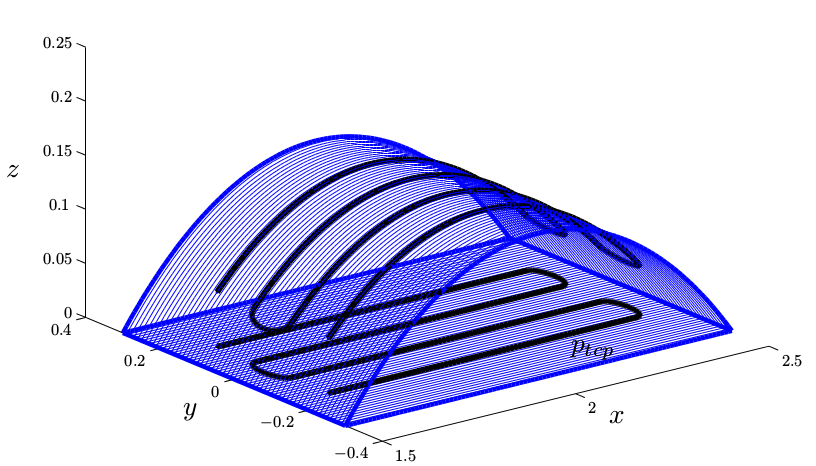
\includegraphics[width=\columnwidth]{figs/planejamento/pal.png}
	\caption{Subregiões de uma superfície.}
	\label{fig::pal}
\end{figure}


A superfície descrita na seção~\ref{modelagem} é uma equação implícita, na forma
$f(x,y,z)=0$. Neste caso, as trajetórias a serem percorridas pelo manipulador
podem ser obtidas através da interseção (cortes) entre planos uniformemente
espaçados e a superfície, o que gerará curvas ao longo da superfície. Uma ideia
semelhante e propícia devido à geometria do rotor, é gerar as curvas a partir da interseção
entre esferas e a superfície. As figuras~\ref{fig::interfrontal}
e~\ref{fig::interiso} mostram duas visões de duas interseções entre esferas e
a pá, onde as interseções estão representadas em vermelho, e as esferas em
azul claro. Os mesmos cortes podem ser observados entre esferas e o modelo
algébrico da pá, em figura~\ref{fig::intergeo}, na qual a pá está representada
em vermelho, as esferas estão em cinza claro, e as interseções são as curvas
sombreadas em cinza na pá.


\begin{figure}[!ht]
	\centering
	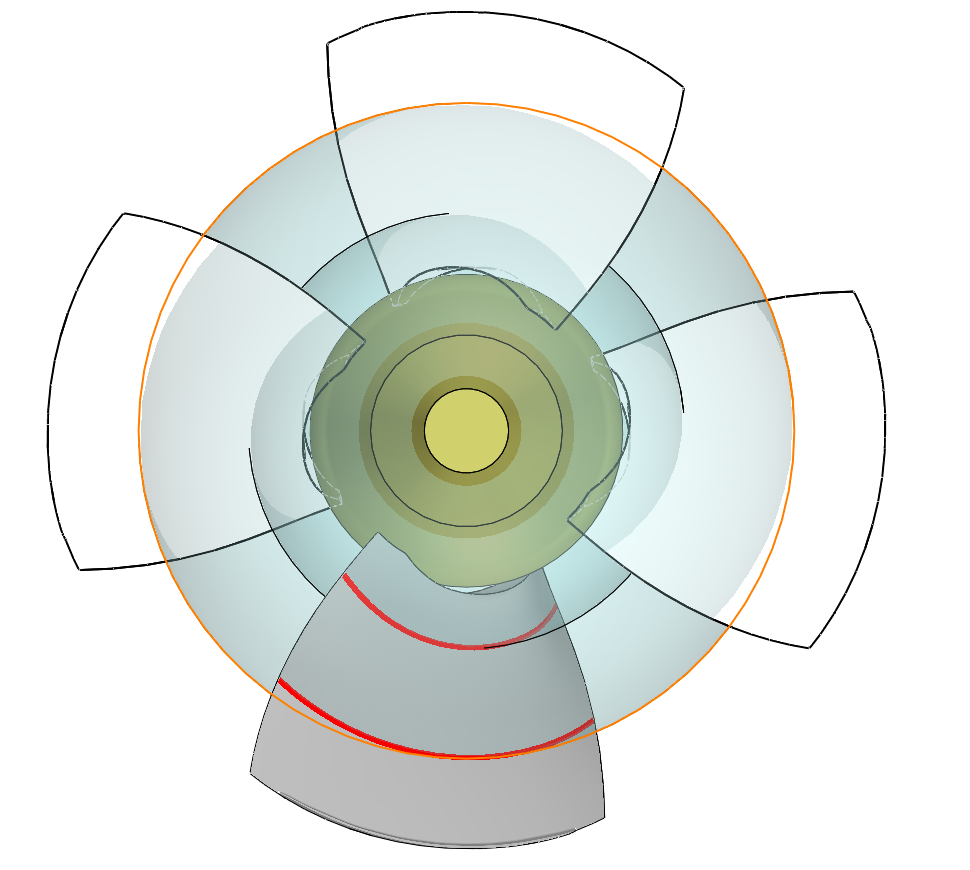
\includegraphics[width=.7\columnwidth]{figs/planejamento/intersecao_frontal.PNG}
	\caption{Interseção esfera-pá, vista frontal.}
	\label{fig::interfrontal}
\end{figure}

\begin{figure}[!ht]
	\centering
	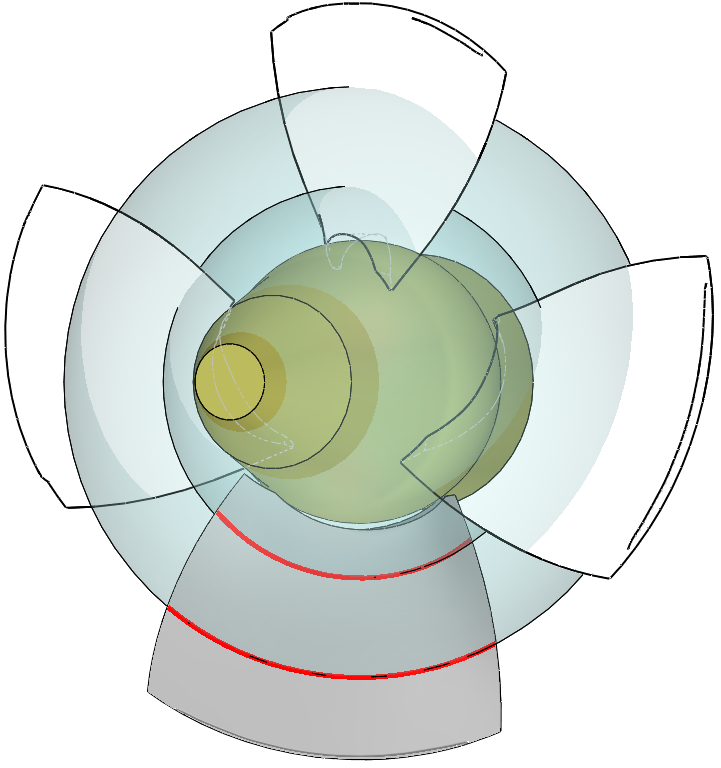
\includegraphics[width=.6\columnwidth]{figs/planejamento/intersecao_iso.PNG}
	\caption{Interseção esfera-pá, vista isométrica.}
	\label{fig::interiso}
\end{figure}

\begin{figure}[!ht]
	\centering
	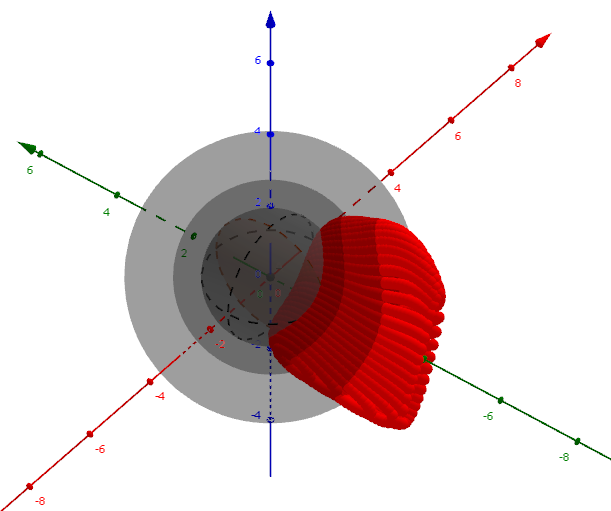
\includegraphics[width=\columnwidth]{figs/planejamento/intersecao_geogebra.png}
	\caption{Interseção esfera-modelo pá.}
	\label{fig::intergeo}
\end{figure}

A interseção de duas superfícies, a superfície da esfera
$g(x,y,z)=x^2+y^2+z^2-R^2=0$ e a superfície da pá $f(x,y,z)=0$, gera o caminho
que deve ser percorrido pelo robô. Porém, resolver algebricamente
$f(x,y,z)=g(x,y,z)$ é muito custoso, haveria a necessidade de
calcular as soluções para os ângulos das juntas do robô posteriormente, e ainda
realizar cáculos de restrição de borda da superfície, já que a função algébrica
encontrada para a pá é contínua e pode ter comportamento estranho fora da
região de interesse. Portanto, foi desenvolvido um método iterativo para a
computação da trajetória do robô de forma que, ao mesmo tempo que o caminho é
criado, os ângulos das juntas são computados, otimizando localmente a variação
dos ângulos das juntas, verificando restrição de ângulo de revestimento, e
bordas.

O método será explicado a partir de um exemplo genérico: suponha a superfície
algébrica da pá em vermelho, o rotor em preto, e a área que pode ser
revestida dada uma base do robô em amarelo, na figura~\ref{fig::vetores_out}.
Nesta etapa de revestimento (robô nesta posição de base), devem ser calculadas
as curvas (trajetórias). É selecionado o ponto central da núvem de
pontos revestidos (em amarelo), e é calculado o ponto mais próximo à superfície,
representado como ponto $B$ da figura~\ref{fig::vetores_out2}.
$\vec{AB}$ é o vetor normal à esfera, igual a $\vec{OB}$ (origem ao ponto B), e $\vec{BC}$ é o vetor normal à superfície
algébrica da pá, calculado como $\nabla{f} = \vec{f_x,f_y,f_z}$. O vetor
tangente $\vec{BD}$, figura~\ref{fig::vetores_in}, pode ser calculado como
produto vetorial entre o vetor normal à superfície da pá com o vetor normal à
esfera, no ponto B: $\vec{BD} = \vec{BC} \times \vec{AB} = \vec{OB} \times
\nabla{f}$. A integral do vetor tangente irá fornecer a trajetória (região
cinza sombreada, ou em vermelho na figura~\ref{fig::interiso}), logo o caminho
(ou trajetória) é calculado por:
$$c = \int \vec{OB} \times \nabla{f} dt$$. 

Em integrações numéricas, deve-se garantir que o novo ponto de cada iteração
pertença à superfície, logo $B' = B + \int_0^t \vec{OB} \times \nabla{f} dt$, onde $t$ é o passo de integração, não é
suficiente, pois deve-se reprojetar o novo ponto $B'$ na superfície da pá. Isso
é feito por uma otimização, enunciada da seguinte forma:
$$min \left \| B-B' \right \|^2$$
$$s.t. f(B')=0$$
E assim garante-se que o novo ponto $B'$ pertence à superfície da pá.

Em cada passo da integração numérica, deve-se computar a solução dos ângulos das
juntas (cinemática inversa) para o revestimento. Caso não haja solução, ou o
ângulo entre avanço do efetuador e normal da pá seja maior que $30^o$, a trajetória está
concluída e a integração é interrompida. Calculam-se os valores dos ângulos das
juntas em cada passo por uma otimização, enunciada da seguinte forma:
$$min -\nabla{f}\cdot x_T$$
$$s.t. \left \| p_T-B \right \|^2=0$$
Onde $x_T$ são as três primeiras linhas da primeira coluna da transformação
homogênea $T_{bB}$ ($b$ é a base do manipulador), pois o vetor de avanço do
efetuador do manipulador é $x=(1,0,0)$, logo a primeira coluna. E $p_T$ são as
três primeiras linhas da quarta coluna da transformação
homogênea $T_{bB'}$, representando a posição do efetuador.

\begin{figure}[!ht]
	\centering
	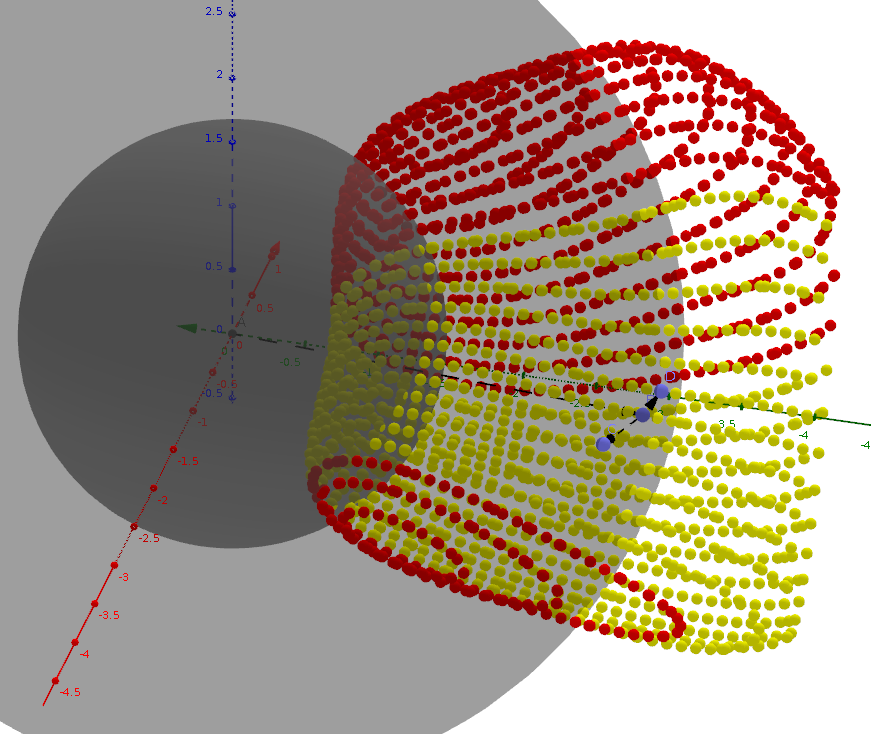
\includegraphics[width=\columnwidth]{figs/planejamento/vetores_out.png}
	\caption{Vetores de interesse na interseção esfera-pá.}
	\label{fig::vetores_out}
\end{figure}

\begin{figure}[!ht]
	\centering
	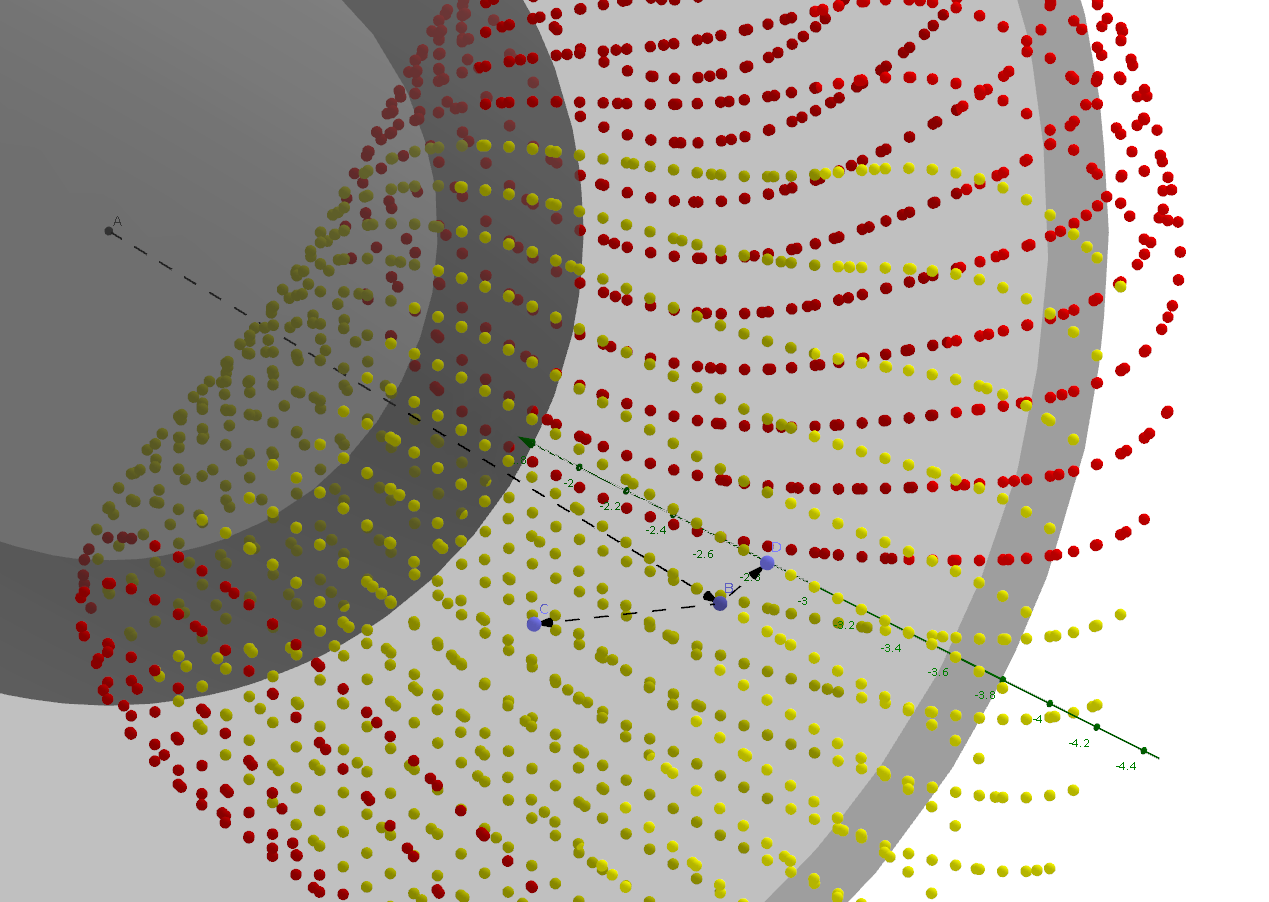
\includegraphics[width=\columnwidth]{figs/planejamento/vetores_out2.png}
	\caption{Vetores de interesse na interseção esfera-pá.}
	\label{fig::vetores_out2}
\end{figure}

\begin{figure}[!ht]
	\centering
	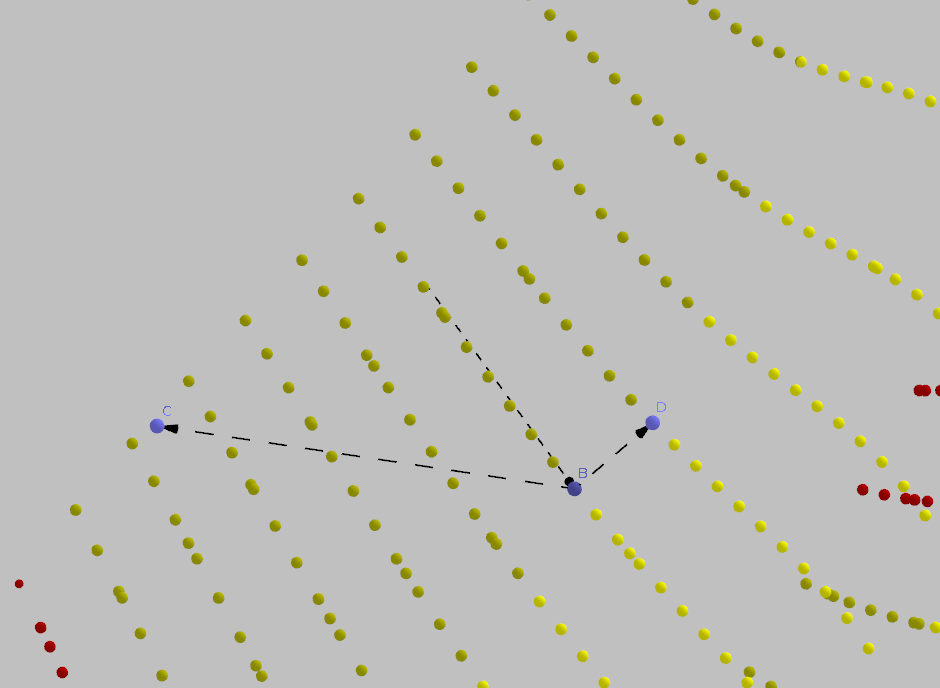
\includegraphics[width=\columnwidth]{figs/planejamento/vetores_in.png}
	\caption{Vetores de interesse na interseção esfera-pá.}
	\label{fig::vetores_in}
\end{figure}

A figura~\ref{fig::path_openrave} mostra duas curvas computadas pelo algoritmo
descrito acima. Os caminhos tem espaçamento exagerado, maior que 3 mm, para
facilitar a visualização. A transição entre os paralelos, no entanto, é
executada por outro algoritmo, que calcula os meridianos do planejamento de
trajetória.

\begin{figure}[!ht]
	\centering
	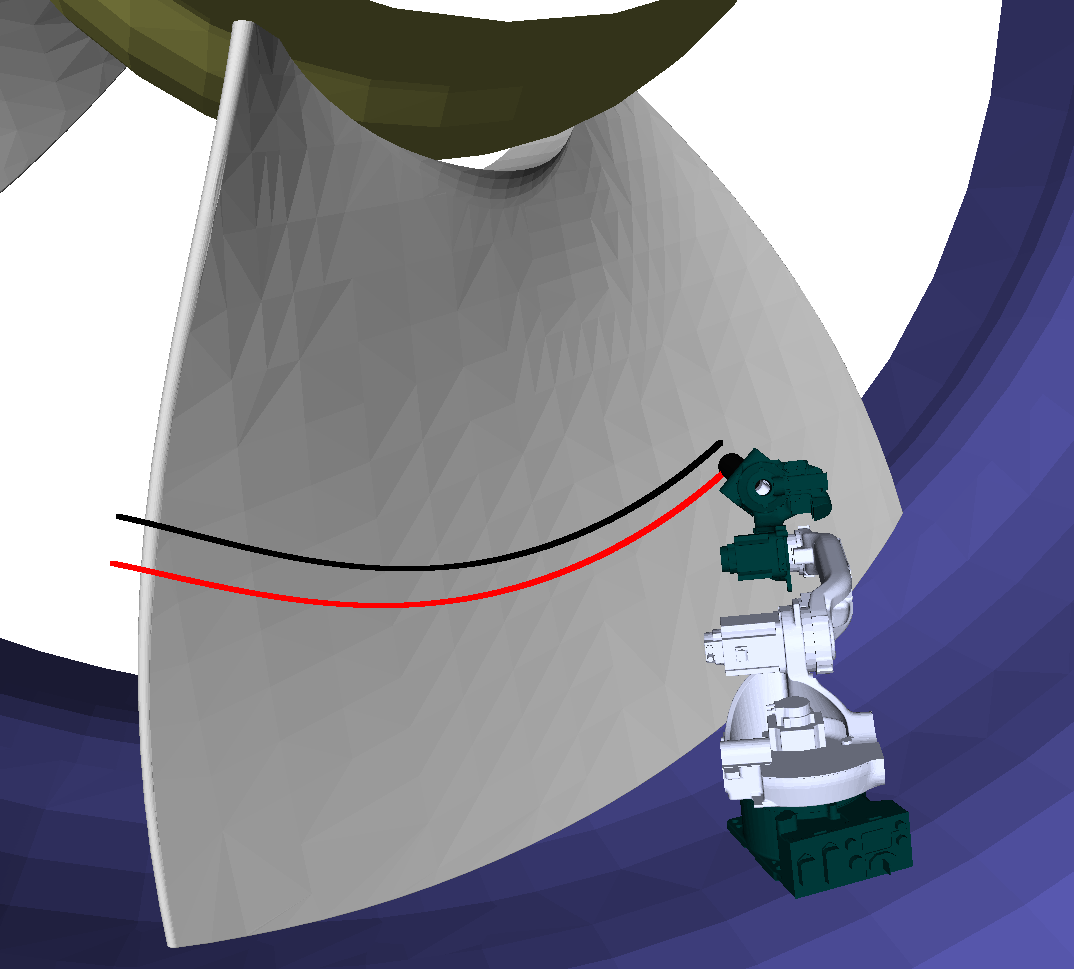
\includegraphics[width=\columnwidth]{figs/planejamento/path_openrave.png}
	\caption{Simulação de trajetória no Openrave.}
	\label{fig::path_openrave}
\end{figure}